\SourceLeaf{441}%
fang der Figur $LL'P'P$ in demselben Sinn umgeht, wie $(1)(2)(3)$, negativ beim entgegengesetzten.
\begin{center}
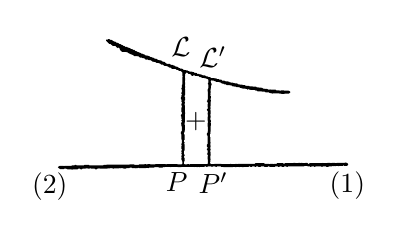
\begin{tikzpicture}[x=.00165in,y=-.00165in]
\path[use as bounding box] (0,0) rectangle (1022,525);
\path[fill=black,even odd rule] (92,424) -- (96,428) -- (98,428) -- (99,429) -- (110,429) -- (111,428) -- (117,428) -- (121,430) -- (133,430) -- (134,431) -- (136,431) -- (137,430) -- (151,430) -- (153,428) -- (159,428) -- (161,430) -- (164,430) -- (166,428) -- (175,428) -- (176,427) -- (182,427) -- (183,428) -- (187,428) -- (188,427) -- (192,427) -- (193,428) -- (204,428) -- (206,430) -- (209,430) -- (211,428) -- (214,428) -- (215,427) -- (218,427) -- (219,428) -- (241,428) -- (242,427) -- (250,427) -- (251,426) -- (259,427) -- (260,428) -- (262,427) -- (276,427) -- (277,426) -- (279,426) -- (280,427) -- (282,426) -- (288,426) -- (289,427) -- (297,428) -- (300,426) -- (308,426) -- (309,425) -- (316,425) -- (317,426) -- (327,426) -- (328,427) -- (330,426) -- (334,426) -- (335,425) -- (337,425) -- (338,426) -- (359,426) -- (360,425) -- (367,426) -- (368,425) -- (383,425) -- (385,423) -- (397,423) -- (399,425) -- (409,425) -- (411,423) -- (416,423) -- (417,422) -- (432,422) -- (433,423) -- (435,423) -- (436,422) -- (454,422) -- (455,423) -- (466,423) -- (467,422) -- (506,422) -- (507,423) -- (509,422) -- (512,422) -- (513,423) -- (515,423) -- (516,422) -- (519,422) -- (520,423) -- (522,423) -- (523,422) -- (536,422) -- (537,421) -- (541,421) -- (542,422) -- (545,422) -- (546,421) -- (557,421) -- (558,422) -- (560,422) -- (561,421) -- (569,421) -- (570,422) -- (573,422) -- (574,421) -- (586,421) -- (587,422) -- (593,422) -- (594,423) -- (622,423) -- (623,422) -- (629,422) -- (630,423) -- (633,423) -- (634,422) -- (640,422) -- (641,423) -- (643,423) -- (644,422) -- (649,422) -- (650,423) -- (655,423) -- (656,422) -- (670,422) -- (671,421) -- (675,421) -- (676,422) -- (680,422) -- (681,421) -- (688,421) -- (689,422) -- (692,422) -- (693,421) -- (699,421) -- (700,422) -- (707,422) -- (708,421) -- (717,421) -- (718,422) -- (728,422) -- (729,421) -- (733,421) -- (734,422) -- (750,422) -- (751,421) -- (759,421) -- (760,422) -- (764,422) -- (765,421) -- (770,421) -- (771,422) -- (777,422) -- (778,421) -- (785,421) -- (786,422) -- (789,422) -- (790,421) -- (838,421) -- (840,419) -- (848,419) -- (850,421) -- (857,421) -- (858,422) -- (860,422) -- (861,421) -- (869,421) -- (870,422) -- (872,422) -- (873,421) -- (891,421) -- (892,422) -- (894,422) -- (895,421) -- (905,421) -- (906,422) -- (912,422) -- (913,421) -- (923,421) -- (924,419) -- (926,420) -- (930,420) -- (931,419) -- (932,420) -- (935,420) -- (936,419) -- (945,420) -- (946,419) -- (956,419) -- (957,418) -- (959,418) -- (960,419) -- (969,419) -- (972,416) -- (972,413) -- (968,410) -- (963,409) -- (962,410) -- (938,410) -- (937,411) -- (933,411) -- (932,410) -- (923,410) -- (922,411) -- (919,411) -- (918,410) -- (910,410) -- (909,411) -- (897,411) -- (896,410) -- (894,411) -- (856,411) -- (854,413) -- (851,413) -- (848,410) -- (843,410) -- (842,411) -- (834,411) -- (833,410) -- (829,410) -- (828,411) -- (826,411) -- (825,410) -- (822,410) -- (821,411) -- (813,411) -- (812,410) -- (807,410) -- (806,411) -- (781,411) -- (779,413) -- (777,413) -- (775,411) -- (757,411) -- (755,413) -- (747,413) -- (746,414) -- (744,414) -- (743,413) -- (736,413) -- (735,414) -- (733,414) -- (732,413) -- (719,413) -- (717,411) -- (691,411) -- (689,413) -- (638,413) -- (637,414) -- (634,414) -- (633,413) -- (631,413) -- (630,414) -- (618,414) -- (617,413) -- (615,413) -- (614,414) -- (588,414) -- (587,413) -- (567,413) -- (566,414) -- (556,414) -- (553,411) -- (553,409) -- (554,408) -- (554,401) -- (555,400) -- (555,398) -- (554,397) -- (554,389) -- (555,388) -- (555,382) -- (554,380) -- (555,379) -- (555,377) -- (553,375) -- (555,371) -- (555,369) -- (554,368) -- (554,362) -- (555,361) -- (554,351) -- (555,350) -- (555,348) -- (554,347) -- (554,332) -- (553,331) -- (553,323) -- (555,320) -- (554,316) -- (555,315) -- (555,298) -- (556,297) -- (556,290) -- (555,289) -- (556,282) -- (554,278) -- (554,274) -- (555,273) -- (555,267) -- (554,266) -- (554,263) -- (555,262) -- (555,251) -- (554,250) -- (554,246) -- (555,245) -- (555,243) -- (554,242) -- (554,239) -- (555,238) -- (555,224) -- (556,223) -- (556,220) -- (555,219) -- (556,208) -- (554,206) -- (554,204) -- (555,203) -- (555,201) -- (554,200) -- (555,198) -- (555,193) -- (554,191) -- (555,190) -- (555,185) -- (556,184) -- (556,176) -- (558,174) -- (558,170) -- (556,168) -- (556,164) -- (555,163) -- (555,162) -- (557,160) -- (560,160) -- (561,161) -- (566,161) -- (567,162) -- (569,162) -- (571,164) -- (582,165) -- (583,166) -- (585,166) -- (590,170) -- (594,170) -- (597,172) -- (602,172) -- (604,174) -- (613,174) -- (614,175) -- (618,175) -- (622,178) -- (627,178) -- (628,179) -- (632,179) -- (633,180) -- (643,181) -- (645,183) -- (648,183) -- (649,184) -- (652,184) -- (653,185) -- (661,185) -- (662,186) -- (665,186) -- (667,188) -- (668,188) -- (670,186) -- (672,188) -- (675,188) -- (676,189) -- (688,189) -- (692,191) -- (696,191) -- (697,193) -- (710,193) -- (711,194) -- (719,194) -- (722,196) -- (732,196) -- (734,198) -- (740,199) -- (741,200) -- (743,200) -- (744,199) -- (763,199) -- (764,200) -- (769,200) -- (770,201) -- (778,201) -- (779,200) -- (792,200) -- (794,199) -- (797,196) -- (797,195) -- (795,193) -- (791,191) -- (778,191) -- (777,190) -- (764,191) -- (763,190) -- (754,190) -- (752,188) -- (737,188) -- (736,187) -- (734,188) -- (730,188) -- (726,186) -- (719,186) -- (718,185) -- (714,185) -- (712,183) -- (710,183) -- (709,182) -- (701,182) -- (700,181) -- (695,181) -- (693,179) -- (683,179) -- (682,178) -- (673,178) -- (672,177) -- (660,176) -- (658,174) -- (652,174) -- (651,173) -- (644,173) -- (643,172) -- (639,172) -- (635,169) -- (628,169) -- (627,168) -- (624,168) -- (623,167) -- (617,167) -- (616,166) -- (613,166) -- (611,164) -- (608,164) -- (607,163) -- (601,163) -- (597,161) -- (590,161) -- (588,158) -- (582,158) -- (580,156) -- (574,156) -- (572,154) -- (567,154) -- (566,153) -- (557,153) -- (553,150) -- (549,150) -- (546,148) -- (542,148) -- (538,145) -- (532,145) -- (526,142) -- (522,142) -- (520,140) -- (514,140) -- (513,138) -- (511,137) -- (506,137) -- (504,135) -- (502,135) -- (501,134) -- (491,133) -- (490,132) -- (487,132) -- (485,130) -- (473,128) -- (468,124) -- (463,124) -- (462,123) -- (460,123) -- (453,118) -- (449,118) -- (445,115) -- (443,115) -- (439,113) -- (435,113) -- (431,110) -- (422,110) -- (421,108) -- (419,108) -- (415,104) -- (409,103) -- (406,100) -- (395,98) -- (392,95) -- (388,95) -- (387,94) -- (385,94) -- (381,91) -- (378,91) -- (377,90) -- (372,89) -- (370,87) -- (366,86) -- (365,85) -- (357,84) -- (354,81) -- (352,81) -- (348,79) -- (345,79) -- (341,76) -- (339,76) -- (336,74) -- (333,74) -- (332,72) -- (327,71) -- (323,67) -- (319,67) -- (317,65) -- (314,65) -- (310,62) -- (303,60) -- (301,58) -- (296,58) -- (294,56) -- (290,55) -- (288,53) -- (286,53) -- (282,50) -- (279,50) -- (277,48) -- (273,46) -- (268,45) -- (265,42) -- (262,42) -- (254,37) -- (251,37) -- (248,35) -- (244,35) -- (243,36) -- (239,36) -- (238,37) -- (238,39) -- (239,41) -- (247,49) -- (250,49) -- (252,50) -- (258,55) -- (266,55) -- (272,62) -- (274,60) -- (275,60) -- (280,64) -- (280,67) -- (286,73) -- (301,74) -- (302,75) -- (304,75) -- (305,77) -- (307,77) -- (311,80) -- (314,80) -- (315,82) -- (317,82) -- (321,84) -- (323,86) -- (333,86) -- (334,87) -- (337,87) -- (341,91) -- (347,91) -- (348,92) -- (354,93) -- (358,97) -- (361,97) -- (363,96) -- (366,98) -- (374,99) -- (379,103) -- (387,104) -- (391,107) -- (397,107) -- (398,108) -- (402,109) -- (405,112) -- (410,112) -- (415,116) -- (421,116) -- (422,117) -- (426,118) -- (430,121) -- (434,121) -- (438,125) -- (448,125) -- (452,128) -- (456,128) -- (459,131) -- (463,131) -- (465,132) -- (469,136) -- (469,146) -- (470,147) -- (470,150) -- (469,151) -- (469,173) -- (468,174) -- (468,182) -- (466,184) -- (466,186) -- (468,188) -- (468,196) -- (466,197) -- (466,200) -- (468,202) -- (468,204) -- (466,206) -- (466,211) -- (465,212) -- (465,216) -- (466,217) -- (466,219) -- (468,221) -- (466,223) -- (466,224) -- (468,226) -- (468,230) -- (466,231) -- (466,235) -- (468,237) -- (468,241) -- (466,243) -- (466,255) -- (468,257) -- (468,262) -- (465,265) -- (465,268) -- (466,269) -- (466,275) -- (468,277) -- (468,279) -- (466,281) -- (466,282) -- (468,284) -- (468,286) -- (466,288) -- (466,290) -- (465,291) -- (466,293) -- (466,298) -- (468,300) -- (468,313) -- (465,316) -- (465,322) -- (466,323) -- (466,338) -- (468,340) -- (468,351) -- (466,352) -- (466,355) -- (468,357) -- (466,359) -- (466,367) -- (468,369) -- (468,372) -- (466,374) -- (466,378) -- (468,379) -- (468,380) -- (466,381) -- (466,383) -- (468,384) -- (468,387) -- (466,389) -- (466,391) -- (468,393) -- (468,394) -- (466,395) -- (466,400) -- (468,402) -- (468,405) -- (469,406) -- (469,413) -- (467,415) -- (455,415) -- (454,414) -- (422,414) -- (421,415) -- (419,415) -- (418,414) -- (388,414) -- (387,415) -- (372,415) -- (371,414) -- (364,414) -- (363,415) -- (359,415) -- (358,414) -- (355,414) -- (354,415) -- (338,415) -- (337,416) -- (324,416) -- (323,415) -- (231,416) -- (229,418) -- (187,418) -- (185,416) -- (173,416) -- (171,418) -- (148,418) -- (146,416) -- (144,416) -- (142,418) -- (134,418) -- (133,419) -- (112,419) -- (111,420) -- (109,420) -- (108,419) -- (98,419) -- (94,421) -- (92,423) -- cycle (482,136) -- (484,136) -- (488,140) -- (492,140) -- (494,141) -- (498,146) -- (501,146) -- (502,145) -- (507,145) -- (508,146) -- (519,147) -- (522,150) -- (526,150) -- (529,152) -- (536,152) -- (537,154) -- (542,154) -- (543,155) -- (545,155) -- (548,158) -- (548,167) -- (547,168) -- (547,171) -- (548,172) -- (548,184) -- (546,188) -- (546,193) -- (547,194) -- (547,216) -- (546,217) -- (546,220) -- (544,222) -- (544,224) -- (546,225) -- (546,228) -- (547,229) -- (547,231) -- (546,232) -- (546,241) -- (547,242) -- (547,245) -- (544,248) -- (544,250) -- (547,254) -- (547,258) -- (546,259) -- (546,263) -- (547,264) -- (547,270) -- (546,271) -- (546,282) -- (547,283) -- (547,289) -- (546,290) -- (546,300) -- (547,301) -- (547,315) -- (546,316) -- (546,319) -- (544,321) -- (544,326) -- (546,328) -- (546,353) -- (544,355) -- (544,361) -- (546,363) -- (546,366) -- (544,368) -- (544,371) -- (547,374) -- (546,376) -- (546,381) -- (544,383) -- (544,384) -- (545,384) -- (547,387) -- (547,390) -- (546,391) -- (546,399) -- (547,400) -- (547,412) -- (545,414) -- (493,414) -- (492,415) -- (490,415) -- (489,414) -- (485,414) -- (484,415) -- (477,415) -- (474,413) -- (474,407) -- (476,405) -- (476,395) -- (474,394) -- (474,391) -- (476,389) -- (476,385) -- (474,384) -- (474,374) -- (476,372) -- (476,354) -- (474,352) -- (476,350) -- (476,348) -- (474,346) -- (474,341) -- (476,340) -- (476,325) -- (474,323) -- (474,319) -- (476,317) -- (476,312) -- (477,311) -- (477,296) -- (476,295) -- (476,288) -- (477,287) -- (477,262) -- (478,261) -- (478,258) -- (477,257) -- (477,236) -- (476,235) -- (476,230) -- (477,229) -- (476,221) -- (478,219) -- (478,217) -- (477,216) -- (478,212) -- (476,210) -- (476,206) -- (478,203) -- (478,201) -- (477,200) -- (478,198) -- (478,187) -- (477,186) -- (477,184) -- (478,183) -- (478,177) -- (477,176) -- (477,173) -- (478,172) -- (478,167) -- (477,166) -- (477,161) -- (478,160) -- (478,152) -- (477,151) -- (477,148) -- (478,147) -- (478,140) -- cycle;
\node[inner sep=0pt,font=\normalsize] at (465,58) {$\mathcal{L}$};
\node[inner sep=0pt,font=\normalsize] at (562,88) {$\mathcal{L}'$};
\node[inner sep=0pt,font=\normalsize] at (510,286) {$+$};
\node[inner sep=0pt,font=\normalsize] at (452,469) {$P$};
\node[inner sep=0pt,font=\normalsize] at (563,473) {$P'$};
\node[inner sep=0pt,font=\normalsize] at (67,482) {$(2)$};
\node[inner sep=0pt,font=\normalsize] at (970,478) {$(1)$};
\end{tikzpicture}
\hfill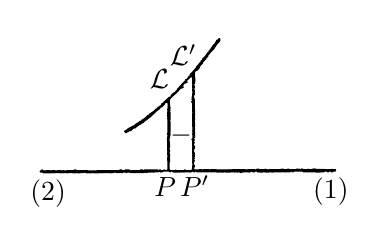
\begin{tikzpicture}[x=.00165in,y=-.00165in]
\path[use as bounding box] (0,0) rectangle (980,539);
\path[fill=black,even odd rule] (936,432) -- (934,429) -- (925,429) -- (924,428) -- (922,428) -- (921,429) -- (908,429) -- (906,430) -- (905,429) -- (873,428) -- (872,427) -- (869,427) -- (868,428) -- (862,428) -- (861,429) -- (854,429) -- (853,428) -- (850,428) -- (849,429) -- (837,429) -- (836,428) -- (831,427) -- (829,429) -- (826,429) -- (825,428) -- (814,428) -- (813,429) -- (794,429) -- (793,428) -- (788,428) -- (787,429) -- (777,429) -- (776,428) -- (768,428) -- (767,429) -- (732,429) -- (731,430) -- (723,429) -- (722,428) -- (720,428) -- (719,429) -- (707,429) -- (706,430) -- (702,428) -- (695,428) -- (692,430) -- (690,430) -- (689,429) -- (668,429) -- (667,430) -- (660,430) -- (659,429) -- (620,429) -- (619,430) -- (617,430) -- (616,429) -- (614,430) -- (612,430) -- (611,429) -- (609,430) -- (573,430) -- (572,429) -- (555,429) -- (554,430) -- (550,430) -- (549,429) -- (534,429) -- (533,430) -- (529,430) -- (528,429) -- (521,429) -- (520,430) -- (507,430) -- (505,428) -- (505,425) -- (507,423) -- (507,417) -- (504,414) -- (505,412) -- (505,407) -- (507,405) -- (507,403) -- (505,401) -- (505,400) -- (507,398) -- (507,397) -- (505,395) -- (507,393) -- (507,379) -- (505,377) -- (505,369) -- (507,368) -- (507,364) -- (508,363) -- (508,360) -- (505,356) -- (505,352) -- (507,350) -- (507,348) -- (505,346) -- (505,344) -- (507,342) -- (507,340) -- (505,338) -- (505,337) -- (508,333) -- (508,315) -- (507,314) -- (507,310) -- (508,309) -- (508,305) -- (507,304) -- (507,301) -- (508,300) -- (508,291) -- (507,290) -- (507,281) -- (508,280) -- (508,273) -- (507,272) -- (507,268) -- (508,267) -- (508,250) -- (507,249) -- (507,215) -- (505,214) -- (505,206) -- (507,204) -- (507,197) -- (508,196) -- (508,194) -- (507,193) -- (507,189) -- (505,187) -- (505,185) -- (507,184) -- (508,179) -- (505,173) -- (508,169) -- (508,165) -- (509,164) -- (509,153) -- (508,152) -- (508,147) -- (507,146) -- (508,138) -- (507,136) -- (511,131) -- (514,131) -- (519,127) -- (519,126) -- (522,123) -- (523,118) -- (532,108) -- (533,104) -- (535,102) -- (536,102) -- (540,97) -- (542,96) -- (543,93) -- (548,88) -- (548,84) -- (552,81) -- (555,76) -- (567,64) -- (568,61) -- (571,58) -- (571,56) -- (574,53) -- (575,53) -- (575,51) -- (582,44) -- (585,39) -- (585,34) -- (583,32) -- (579,32) -- (579,33) -- (576,36) -- (574,36) -- (572,38) -- (572,40) -- (570,42) -- (568,46) -- (559,56) -- (559,58) -- (555,62) -- (554,65) -- (549,70) -- (548,73) -- (543,77) -- (543,79) -- (540,82) -- (538,86) -- (530,93) -- (529,97) -- (525,100) -- (525,102) -- (517,111) -- (517,112) -- (511,118) -- (510,121) -- (508,123) -- (507,123) -- (507,125) -- (502,130) -- (502,131) -- (492,141) -- (491,145) -- (486,149) -- (485,152) -- (481,156) -- (478,157) -- (478,159) -- (458,180) -- (458,181) -- (453,186) -- (453,188) -- (449,192) -- (448,192) -- (448,193) -- (445,196) -- (442,197) -- (435,204) -- (434,204) -- (434,208) -- (433,209) -- (430,209) -- (428,211) -- (427,211) -- (408,229) -- (405,230) -- (405,233) -- (402,236) -- (401,236) -- (398,239) -- (395,240) -- (391,245) -- (388,246) -- (380,254) -- (376,256) -- (373,259) -- (371,259) -- (367,264) -- (364,265) -- (356,273) -- (353,274) -- (350,277) -- (347,278) -- (344,282) -- (341,282) -- (334,288) -- (332,288) -- (321,297) -- (318,297) -- (313,301) -- (306,304) -- (297,311) -- (293,313) -- (293,316) -- (297,320) -- (300,320) -- (302,318) -- (304,318) -- (307,315) -- (310,315) -- (314,313) -- (317,310) -- (318,310) -- (320,307) -- (328,305) -- (332,300) -- (334,300) -- (340,295) -- (344,294) -- (344,293) -- (346,291) -- (348,291) -- (350,289) -- (351,289) -- (358,282) -- (362,281) -- (365,277) -- (372,273) -- (382,263) -- (383,263) -- (390,255) -- (391,255) -- (396,250) -- (398,250) -- (398,249) -- (400,248) -- (404,243) -- (407,242) -- (416,233) -- (418,229) -- (420,228) -- (423,228) -- (424,229) -- (424,232) -- (425,233) -- (425,238) -- (424,239) -- (425,243) -- (423,247) -- (423,249) -- (424,250) -- (424,254) -- (423,255) -- (423,270) -- (424,271) -- (424,273) -- (423,274) -- (423,276) -- (424,277) -- (424,319) -- (423,320) -- (423,325) -- (424,326) -- (424,330) -- (423,331) -- (423,335) -- (422,336) -- (422,338) -- (423,339) -- (423,341) -- (422,342) -- (422,344) -- (423,345) -- (423,375) -- (424,376) -- (424,378) -- (423,379) -- (423,386) -- (424,387) -- (424,393) -- (423,394) -- (423,403) -- (424,404) -- (424,429) -- (422,432) -- (418,432) -- (417,430) -- (413,430) -- (412,432) -- (405,432) -- (403,430) -- (400,430) -- (398,432) -- (397,432) -- (395,430) -- (354,430) -- (352,432) -- (350,432) -- (349,430) -- (342,430) -- (340,432) -- (315,432) -- (314,433) -- (312,433) -- (308,430) -- (296,430) -- (294,432) -- (287,432) -- (286,430) -- (279,430) -- (277,432) -- (260,432) -- (259,433) -- (257,432) -- (253,432) -- (252,433) -- (250,432) -- (210,432) -- (209,433) -- (183,433) -- (182,432) -- (149,432) -- (147,430) -- (141,430) -- (139,432) -- (119,432) -- (118,433) -- (111,433) -- (110,432) -- (107,432) -- (106,433) -- (102,433) -- (101,432) -- (90,432) -- (89,433) -- (84,433) -- (83,432) -- (74,432) -- (73,433) -- (69,433) -- (68,432) -- (48,433) -- (45,430) -- (43,430) -- (40,433) -- (39,433) -- (36,436) -- (36,437) -- (39,440) -- (45,440) -- (47,442) -- (74,442) -- (75,441) -- (78,441) -- (79,442) -- (82,442) -- (83,441) -- (97,441) -- (98,442) -- (103,442) -- (104,441) -- (107,441) -- (108,442) -- (110,442) -- (111,441) -- (117,441) -- (118,442) -- (122,442) -- (123,441) -- (136,441) -- (137,442) -- (146,442) -- (147,441) -- (150,441) -- (151,442) -- (159,442) -- (160,441) -- (170,441) -- (171,440) -- (177,441) -- (178,442) -- (182,442) -- (183,441) -- (185,442) -- (194,442) -- (195,441) -- (199,441) -- (200,442) -- (217,442) -- (218,441) -- (224,441) -- (225,442) -- (228,442) -- (229,441) -- (249,441) -- (250,442) -- (253,442) -- (254,441) -- (262,441) -- (263,440) -- (267,440) -- (268,441) -- (279,441) -- (280,440) -- (282,441) -- (289,441) -- (290,440) -- (297,440) -- (298,441) -- (301,441) -- (302,440) -- (310,440) -- (311,441) -- (354,441) -- (355,440) -- (358,440) -- (359,441) -- (362,441) -- (363,440) -- (375,440) -- (376,439) -- (378,439) -- (379,440) -- (384,440) -- (385,439) -- (398,439) -- (400,437) -- (403,440) -- (405,439) -- (409,439) -- (411,437) -- (429,437) -- (431,439) -- (433,439) -- (435,437) -- (438,437) -- (442,440) -- (462,440) -- (463,439) -- (465,439) -- (466,440) -- (468,439) -- (471,439) -- (472,440) -- (475,440) -- (476,439) -- (490,439) -- (491,440) -- (493,440) -- (494,439) -- (497,439) -- (499,437) -- (501,437) -- (503,439) -- (507,439) -- (509,437) -- (511,437) -- (513,439) -- (569,439) -- (571,438) -- (574,440) -- (581,440) -- (582,439) -- (584,439) -- (585,440) -- (595,440) -- (596,439) -- (599,439) -- (600,440) -- (615,440) -- (616,439) -- (626,439) -- (627,440) -- (634,439) -- (635,440) -- (639,440) -- (640,439) -- (643,439) -- (645,441) -- (648,441) -- (649,440) -- (655,440) -- (656,439) -- (670,439) -- (671,440) -- (674,440) -- (678,437) -- (680,437) -- (682,439) -- (689,439) -- (691,437) -- (695,437) -- (698,440) -- (700,439) -- (703,439) -- (704,440) -- (713,440) -- (714,439) -- (720,439) -- (721,440) -- (726,440) -- (727,439) -- (729,440) -- (731,440) -- (732,439) -- (740,439) -- (741,440) -- (745,440) -- (746,439) -- (797,439) -- (799,437) -- (801,437) -- (803,439) -- (806,439) -- (808,437) -- (834,437) -- (836,439) -- (873,439) -- (874,440) -- (888,440) -- (889,439) -- (899,439) -- (901,437) -- (907,437) -- (909,439) -- (913,439) -- (915,437) -- (919,437) -- (921,439) -- (926,439) -- (927,437) -- (933,437) -- (936,434) -- cycle (496,150) -- (499,153) -- (499,171) -- (500,172) -- (499,174) -- (499,182) -- (500,183) -- (500,185) -- (499,186) -- (499,193) -- (500,194) -- (500,199) -- (499,200) -- (499,208) -- (497,210) -- (497,211) -- (499,213) -- (497,215) -- (497,218) -- (499,219) -- (499,221) -- (496,224) -- (497,228) -- (499,229) -- (499,255) -- (500,256) -- (500,258) -- (499,259) -- (499,286) -- (500,287) -- (499,289) -- (499,292) -- (500,293) -- (499,295) -- (499,300) -- (500,301) -- (500,311) -- (499,312) -- (500,320) -- (499,321) -- (499,324) -- (500,325) -- (500,335) -- (497,338) -- (497,340) -- (499,342) -- (499,359) -- (500,360) -- (499,362) -- (499,384) -- (500,385) -- (499,387) -- (499,390) -- (500,391) -- (500,393) -- (499,394) -- (499,396) -- (500,397) -- (500,399) -- (499,400) -- (499,403) -- (500,404) -- (499,406) -- (499,411) -- (500,412) -- (500,418) -- (499,419) -- (499,429) -- (496,432) -- (480,432) -- (478,430) -- (475,430) -- (473,432) -- (451,432) -- (449,430) -- (447,432) -- (434,432) -- (431,429) -- (431,409) -- (432,408) -- (432,395) -- (431,394) -- (432,392) -- (432,382) -- (431,381) -- (431,378) -- (432,377) -- (432,370) -- (431,369) -- (431,365) -- (432,364) -- (432,355) -- (431,354) -- (432,346) -- (431,345) -- (431,336) -- (432,335) -- (432,328) -- (434,326) -- (434,321) -- (432,319) -- (434,317) -- (434,285) -- (432,283) -- (432,282) -- (434,280) -- (434,257) -- (432,255) -- (432,253) -- (434,251) -- (432,249) -- (432,248) -- (434,246) -- (434,241) -- (432,239) -- (432,230) -- (431,229) -- (432,218) -- (442,207) -- (443,207) -- (453,198) -- (454,198) -- (454,196) -- (456,194) -- (459,193) -- (459,191) -- (465,185) -- (468,185) -- (472,183) -- (474,181) -- (471,176) -- (474,174) -- (474,172) -- (476,170) -- (481,169) -- (485,166) -- (485,164) -- (484,163) -- (485,160) -- cycle;
\node[inner sep=0pt,font=\normalsize] at (400,155) {$\mathcal{L}$};
\node[inner sep=0pt,font=\normalsize] at (472,82) {$\mathcal{L}'$};
\node[inner sep=0pt,font=\normalsize] at (466,326) {$-$};
\node[inner sep=0pt,font=\normalsize] at (417,484) {$P$};
\node[inner sep=0pt,font=\normalsize] at (507,482) {$P'$};
\node[inner sep=0pt,font=\normalsize] at (62,502) {$(2)$};
\node[inner sep=0pt,font=\normalsize] at (920,497) {$(1)$};
\end{tikzpicture}
\hfill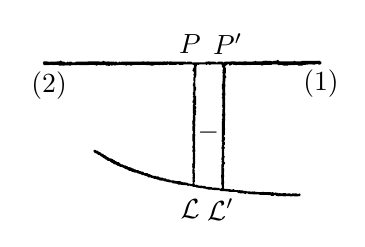
\begin{tikzpicture}[x=.00165in,y=-.00165in]
\path[use as bounding box] (0,0) rectangle (938,581);
\path[fill=black,even odd rule] (827,510) -- (828,505) -- (824,503) -- (822,504) -- (817,504) -- (816,503) -- (811,503) -- (810,504) -- (808,503) -- (803,503) -- (802,504) -- (798,504) -- (797,503) -- (789,503) -- (788,504) -- (786,504) -- (783,502) -- (775,502) -- (774,503) -- (762,502) -- (760,503) -- (756,500) -- (754,502) -- (752,500) -- (748,502) -- (744,499) -- (742,499) -- (741,500) -- (738,500) -- (737,499) -- (718,499) -- (717,498) -- (711,498) -- (710,499) -- (698,499) -- (697,498) -- (690,498) -- (689,497) -- (686,497) -- (685,498) -- (683,497) -- (677,498) -- (676,497) -- (665,497) -- (663,495) -- (654,495) -- (653,494) -- (645,494) -- (644,493) -- (642,493) -- (641,494) -- (639,493) -- (629,493) -- (625,490) -- (623,490) -- (622,491) -- (616,491) -- (615,490) -- (597,489) -- (595,487) -- (595,483) -- (596,482) -- (596,480) -- (595,479) -- (595,474) -- (596,473) -- (596,466) -- (595,465) -- (595,454) -- (596,453) -- (596,445) -- (595,444) -- (595,440) -- (596,439) -- (596,427) -- (594,425) -- (594,424) -- (595,423) -- (595,418) -- (596,417) -- (596,415) -- (599,412) -- (598,409) -- (596,407) -- (596,395) -- (598,393) -- (598,391) -- (596,389) -- (596,377) -- (595,376) -- (596,374) -- (596,367) -- (598,366) -- (598,363) -- (596,362) -- (596,357) -- (598,355) -- (598,347) -- (596,345) -- (596,343) -- (598,342) -- (598,337) -- (599,336) -- (599,334) -- (596,331) -- (596,327) -- (598,325) -- (598,310) -- (599,309) -- (599,306) -- (598,305) -- (598,284) -- (599,283) -- (599,266) -- (600,265) -- (600,263) -- (599,262) -- (599,256) -- (598,255) -- (598,252) -- (599,251) -- (599,226) -- (598,225) -- (598,223) -- (599,222) -- (599,211) -- (598,210) -- (598,207) -- (600,205) -- (600,199) -- (599,198) -- (599,180) -- (600,179) -- (599,164) -- (600,163) -- (600,156) -- (599,154) -- (603,150) -- (600,144) -- (600,139) -- (601,138) -- (601,122) -- (599,120) -- (599,117) -- (608,110) -- (609,110) -- (613,115) -- (615,115) -- (617,113) -- (619,113) -- (621,111) -- (623,111) -- (625,113) -- (629,113) -- (630,114) -- (635,114) -- (636,113) -- (650,113) -- (651,114) -- (664,114) -- (665,113) -- (673,113) -- (674,114) -- (676,114) -- (677,113) -- (707,113) -- (710,115) -- (712,115) -- (713,114) -- (717,114) -- (718,113) -- (740,113) -- (741,111) -- (758,111) -- (761,114) -- (764,114) -- (765,113) -- (770,113) -- (771,114) -- (775,114) -- (776,115) -- (789,115) -- (790,114) -- (800,114) -- (801,113) -- (804,113) -- (805,114) -- (809,114) -- (810,113) -- (819,113) -- (821,115) -- (833,115) -- (837,113) -- (850,112) -- (851,111) -- (864,111) -- (865,112) -- (872,112) -- (873,111) -- (879,110) -- (883,112) -- (887,112) -- (891,109) -- (891,105) -- (889,102) -- (887,102) -- (885,100) -- (883,100) -- (882,101) -- (831,101) -- (830,102) -- (812,102) -- (811,101) -- (808,101) -- (807,102) -- (764,102) -- (760,98) -- (758,98) -- (756,100) -- (745,101) -- (744,102) -- (740,102) -- (739,101) -- (725,101) -- (724,100) -- (714,101) -- (713,102) -- (693,102) -- (692,101) -- (690,101) -- (689,102) -- (684,102) -- (683,103) -- (665,103) -- (664,102) -- (656,102) -- (655,103) -- (645,103) -- (644,102) -- (642,103) -- (630,103) -- (629,102) -- (617,102) -- (616,103) -- (598,103) -- (596,105) -- (593,105) -- (591,103) -- (577,103) -- (576,105) -- (571,105) -- (569,103) -- (552,103) -- (551,102) -- (548,102) -- (547,103) -- (541,103) -- (539,105) -- (502,105) -- (501,106) -- (499,106) -- (496,103) -- (484,103) -- (482,105) -- (481,105) -- (479,103) -- (436,103) -- (435,102) -- (431,102) -- (430,103) -- (426,103) -- (425,102) -- (422,102) -- (421,103) -- (417,103) -- (416,102) -- (413,102) -- (412,103) -- (367,103) -- (366,102) -- (364,102) -- (363,103) -- (354,103) -- (353,102) -- (349,102) -- (348,103) -- (285,103) -- (283,105) -- (281,105) -- (280,103) -- (277,103) -- (276,105) -- (271,105) -- (270,103) -- (266,103) -- (264,105) -- (262,103) -- (246,103) -- (245,102) -- (243,102) -- (242,103) -- (236,103) -- (235,102) -- (232,102) -- (231,101) -- (228,101) -- (226,103) -- (218,103) -- (217,102) -- (204,102) -- (203,103) -- (201,102) -- (183,102) -- (182,103) -- (146,103) -- (145,105) -- (134,105) -- (132,103) -- (128,103) -- (126,105) -- (124,105) -- (122,103) -- (121,103) -- (119,105) -- (113,105) -- (111,103) -- (106,103) -- (105,102) -- (103,102) -- (101,100) -- (99,100) -- (97,102) -- (89,102) -- (88,103) -- (68,103) -- (66,105) -- (64,103) -- (60,103) -- (59,102) -- (49,102) -- (48,103) -- (48,105) -- (46,106) -- (46,108) -- (48,110) -- (48,112) -- (50,114) -- (64,114) -- (65,113) -- (78,113) -- (79,114) -- (81,114) -- (82,113) -- (93,113) -- (96,115) -- (101,115) -- (102,114) -- (104,115) -- (111,115) -- (112,114) -- (131,115) -- (132,114) -- (138,114) -- (139,113) -- (141,113) -- (142,114) -- (144,114) -- (145,113) -- (147,114) -- (149,114) -- (150,113) -- (156,113) -- (157,114) -- (184,114) -- (185,113) -- (202,113) -- (203,114) -- (207,114) -- (208,115) -- (210,115) -- (213,113) -- (216,113) -- (217,114) -- (230,114) -- (231,113) -- (235,113) -- (238,115) -- (244,115) -- (246,117) -- (247,117) -- (250,114) -- (253,114) -- (254,115) -- (257,115) -- (258,114) -- (263,114) -- (264,115) -- (266,115) -- (267,114) -- (274,114) -- (275,113) -- (289,113) -- (290,114) -- (293,114) -- (295,113) -- (298,115) -- (300,115) -- (301,114) -- (311,114) -- (312,115) -- (315,115) -- (316,114) -- (322,114) -- (323,113) -- (334,113) -- (335,114) -- (338,114) -- (339,113) -- (359,113) -- (360,114) -- (372,114) -- (373,115) -- (381,115) -- (382,114) -- (387,114) -- (388,113) -- (396,113) -- (397,114) -- (402,114) -- (403,113) -- (407,113) -- (408,114) -- (410,114) -- (411,113) -- (423,113) -- (425,111) -- (428,111) -- (430,113) -- (451,113) -- (453,111) -- (458,111) -- (460,113) -- (471,113) -- (473,111) -- (500,111) -- (502,113) -- (503,113) -- (505,115) -- (505,116) -- (504,117) -- (504,121) -- (501,125) -- (501,128) -- (500,129) -- (500,130) -- (504,134) -- (504,141) -- (503,142) -- (503,144) -- (504,145) -- (504,150) -- (503,151) -- (503,161) -- (504,162) -- (504,165) -- (503,166) -- (503,169) -- (501,171) -- (501,177) -- (503,178) -- (503,195) -- (501,197) -- (501,203) -- (503,205) -- (503,207) -- (501,208) -- (501,211) -- (503,212) -- (503,218) -- (501,220) -- (501,223) -- (500,224) -- (500,226) -- (503,230) -- (503,232) -- (501,234) -- (501,260) -- (503,262) -- (503,263) -- (501,265) -- (501,281) -- (499,284) -- (500,286) -- (500,294) -- (501,295) -- (501,297) -- (500,298) -- (500,312) -- (501,313) -- (501,322) -- (500,323) -- (500,344) -- (501,345) -- (501,358) -- (500,359) -- (500,365) -- (501,366) -- (501,370) -- (500,371) -- (500,376) -- (501,377) -- (501,394) -- (500,396) -- (501,397) -- (501,411) -- (499,415) -- (500,417) -- (499,421) -- (500,422) -- (500,426) -- (501,427) -- (501,429) -- (500,430) -- (500,443) -- (501,444) -- (501,448) -- (500,449) -- (501,451) -- (501,453) -- (500,454) -- (500,457) -- (501,458) -- (500,468) -- (501,469) -- (501,472) -- (498,475) -- (494,474) -- (493,473) -- (488,473) -- (486,471) -- (483,471) -- (482,470) -- (471,469) -- (470,468) -- (465,468) -- (464,466) -- (447,465) -- (443,463) -- (434,463) -- (432,461) -- (422,460) -- (419,457) -- (412,457) -- (409,455) -- (403,455) -- (402,454) -- (400,454) -- (396,451) -- (389,451) -- (388,450) -- (378,449) -- (377,447) -- (374,447) -- (370,444) -- (366,444) -- (363,441) -- (354,441) -- (350,437) -- (345,437) -- (342,435) -- (339,435) -- (335,432) -- (329,432) -- (327,430) -- (324,430) -- (322,428) -- (320,428) -- (315,425) -- (312,425) -- (310,423) -- (305,423) -- (302,420) -- (299,420) -- (297,418) -- (293,418) -- (288,415) -- (284,415) -- (276,408) -- (272,408) -- (268,405) -- (266,405) -- (264,402) -- (261,402) -- (258,399) -- (256,399) -- (254,397) -- (247,396) -- (245,394) -- (245,393) -- (241,392) -- (235,387) -- (233,387) -- (229,383) -- (224,382) -- (221,378) -- (219,378) -- (215,376) -- (212,373) -- (208,373) -- (206,371) -- (201,371) -- (200,372) -- (200,376) -- (204,380) -- (209,382) -- (216,387) -- (219,387) -- (223,391) -- (225,391) -- (230,396) -- (232,396) -- (237,400) -- (240,401) -- (243,404) -- (247,404) -- (249,405) -- (253,409) -- (257,410) -- (261,414) -- (267,415) -- (273,419) -- (277,419) -- (280,422) -- (284,422) -- (286,424) -- (289,424) -- (297,429) -- (302,430) -- (307,434) -- (314,435) -- (315,437) -- (321,438) -- (325,440) -- (331,440) -- (333,442) -- (339,443) -- (340,444) -- (343,444) -- (347,447) -- (352,447) -- (357,450) -- (361,450) -- (366,454) -- (373,454) -- (375,456) -- (378,456) -- (385,459) -- (390,459) -- (392,461) -- (397,461) -- (399,463) -- (403,463) -- (404,464) -- (412,464) -- (414,466) -- (419,466) -- (420,467) -- (422,467) -- (423,468) -- (427,468) -- (428,469) -- (436,469) -- (440,472) -- (455,474) -- (456,476) -- (465,476) -- (466,477) -- (483,478) -- (487,481) -- (488,481) -- (489,479) -- (492,479) -- (494,481) -- (499,481) -- (503,483) -- (510,483) -- (512,485) -- (517,485) -- (518,486) -- (523,486) -- (524,487) -- (533,487) -- (534,488) -- (539,488) -- (541,490) -- (546,490) -- (547,491) -- (565,492) -- (566,493) -- (569,493) -- (570,492) -- (572,493) -- (582,493) -- (586,496) -- (600,496) -- (601,497) -- (610,497) -- (611,498) -- (636,498) -- (637,499) -- (637,502) -- (644,502) -- (645,503) -- (649,503) -- (651,502) -- (652,503) -- (657,503) -- (659,505) -- (661,505) -- (663,503) -- (666,503) -- (668,502) -- (671,505) -- (682,505) -- (683,506) -- (703,506) -- (704,507) -- (730,507) -- (731,508) -- (737,508) -- (739,510) -- (746,510) -- (748,508) -- (752,508) -- (754,510) -- (756,510) -- (760,512) -- (762,511) -- (776,511) -- (777,512) -- (782,512) -- (783,511) -- (796,511) -- (797,512) -- (808,511) -- (809,512) -- (821,512) -- (822,511) -- (826,511) -- cycle (516,111) -- (518,113) -- (519,113) -- (521,111) -- (540,111) -- (542,113) -- (543,113) -- (545,111) -- (550,111) -- (552,113) -- (554,113) -- (556,111) -- (587,111) -- (589,113) -- (589,118) -- (592,121) -- (592,123) -- (593,124) -- (592,128) -- (591,129) -- (592,131) -- (592,133) -- (591,134) -- (591,138) -- (592,139) -- (591,166) -- (592,168) -- (589,172) -- (589,186) -- (591,188) -- (591,199) -- (589,201) -- (589,204) -- (591,206) -- (591,209) -- (589,211) -- (589,213) -- (591,215) -- (591,235) -- (589,236) -- (589,237) -- (591,239) -- (591,243) -- (592,244) -- (592,246) -- (591,247) -- (591,262) -- (589,264) -- (589,266) -- (591,268) -- (591,276) -- (589,278) -- (589,280) -- (591,282) -- (589,284) -- (589,342) -- (588,344) -- (591,347) -- (591,348) -- (589,350) -- (591,354) -- (589,356) -- (589,362) -- (588,363) -- (588,366) -- (589,367) -- (589,394) -- (588,395) -- (588,400) -- (589,401) -- (589,405) -- (588,406) -- (589,408) -- (589,414) -- (588,415) -- (588,447) -- (587,448) -- (588,470) -- (587,471) -- (587,473) -- (588,474) -- (588,478) -- (589,479) -- (589,486) -- (587,488) -- (582,488) -- (581,486) -- (573,486) -- (572,485) -- (559,485) -- (558,484) -- (555,484) -- (554,483) -- (541,483) -- (539,481) -- (537,481) -- (536,480) -- (529,480) -- (528,479) -- (518,479) -- (517,478) -- (515,478) -- (513,476) -- (509,478) -- (506,474) -- (506,469) -- (507,468) -- (507,461) -- (506,460) -- (507,458) -- (507,441) -- (506,440) -- (507,432) -- (506,431) -- (506,427) -- (507,426) -- (507,415) -- (508,414) -- (508,398) -- (507,397) -- (508,395) -- (508,381) -- (507,380) -- (507,377) -- (509,375) -- (508,369) -- (507,368) -- (508,366) -- (508,362) -- (507,361) -- (507,358) -- (508,357) -- (508,344) -- (507,343) -- (507,341) -- (508,340) -- (508,335) -- (507,334) -- (507,332) -- (508,331) -- (508,327) -- (509,326) -- (509,324) -- (507,322) -- (507,320) -- (508,319) -- (508,298) -- (509,297) -- (509,294) -- (508,293) -- (509,271) -- (508,270) -- (508,268) -- (509,267) -- (509,265) -- (511,264) -- (511,261) -- (509,259) -- (511,257) -- (511,251) -- (509,249) -- (511,247) -- (511,243) -- (512,242) -- (512,241) -- (509,238) -- (509,235) -- (511,233) -- (511,208) -- (509,207) -- (509,191) -- (511,189) -- (511,181) -- (509,179) -- (509,168) -- (508,167) -- (508,164) -- (509,163) -- (509,152) -- (511,150) -- (511,146) -- (512,145) -- (512,118) -- (513,117) -- (513,114) -- cycle;
\node[inner sep=0pt,font=\normalsize] at (492,50) {$P$};
\node[inner sep=0pt,font=\normalsize] at (607,49) {$P'$};
\node[inner sep=0pt,font=\normalsize] at (548,319) {$-$};
\node[inner sep=0pt,font=\normalsize] at (493,549) {$\mathcal{L}$};
\node[inner sep=0pt,font=\normalsize] at (585,552) {$\mathcal{L}'$};
\node[inner sep=0pt,font=\normalsize] at (65,176) {$(2)$};
\node[inner sep=0pt,font=\normalsize] at (890,169) {$(1)$};
\end{tikzpicture}

\end{center}
\noindent\hspace*{1.2em}Man denke sich nun ein endliches Stück der Linie von $L$ nach $L'$ und nenne $\varphi$, $\varphi'$ die an beiden Endpunkten geltenden Werthe des Winkels, so ist
\[
\varphi'=\varphi+\operatorname{Area}LL'P'P,
\]
das Zeichen der Area eben so verstanden.

Man nehme nun ferner an, dass von dem Anfangspunkte auf der krummen Fläche unzählige andere kürzeste Linien auslaufen und nenne den Winkel, den indefinite das erste Element mit dem ersten Elemente der ersten Linie links herum macht, $A$; durch das zweite Ende dieser verschiedenen krummen Linien sei eine krumme Linie gezogen, von der wir vorerst unentschieden lassen, ob sie eine kürzeste Linie sei oder nicht. Setzen wir nun, dass indefinite für jede dieser Linien das, was für die erste $\varphi$, $\varphi'$ war, durch $\psi$, $\psi'$ bezeichnet wird, so ist $\psi'-\psi$ auf ähnliche Weise auf der Hülfskugel durch den Raum $LL'P'P$ darzustellen, und da offenbar $\psi=\varphi-A$ wird, so ist der Raum
\[
\begin{aligned}
LL'_1P'_1P'L'L&=\psi'-\psi-\varphi'+\varphi\\
&=\psi'-\varphi'+A\\
&=LL'_1L'L+L'L'_1P'_1P'.
\end{aligned}
\]
\begin{center}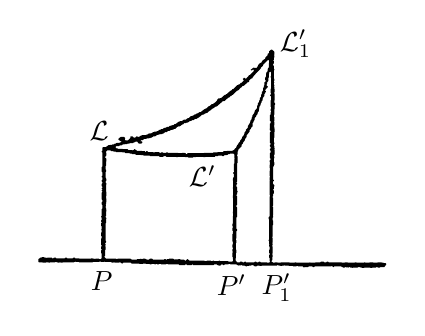
\begin{tikzpicture}[x=.002in,y=-.002in]
\path[use as bounding box] (0,0) rectangle (924,700);
\path[fill=black,even odd rule] (897,592) -- (897,591) -- (895,589) -- (891,589) -- (890,588) -- (886,588) -- (885,587) -- (876,587) -- (875,588) -- (865,588) -- (864,587) -- (856,587) -- (855,588) -- (845,588) -- (844,587) -- (842,587) -- (841,588) -- (823,588) -- (822,587) -- (819,587) -- (818,588) -- (801,588) -- (800,587) -- (794,587) -- (793,588) -- (786,588) -- (785,587) -- (753,587) -- (751,585) -- (749,585) -- (747,587) -- (742,587) -- (740,585) -- (734,585) -- (732,587) -- (720,587) -- (719,588) -- (707,588) -- (706,587) -- (704,588) -- (672,588) -- (671,587) -- (669,587) -- (668,588) -- (655,588) -- (654,587) -- (634,587) -- (633,588) -- (619,587) -- (618,588) -- (614,588) -- (609,584) -- (612,581) -- (612,574) -- (613,573) -- (613,569) -- (612,568) -- (612,565) -- (613,564) -- (613,548) -- (612,547) -- (612,544) -- (613,543) -- (613,541) -- (612,540) -- (612,538) -- (613,537) -- (613,527) -- (612,526) -- (612,523) -- (613,522) -- (613,494) -- (614,493) -- (614,483) -- (613,482) -- (613,475) -- (614,474) -- (614,472) -- (613,471) -- (614,469) -- (614,449) -- (613,448) -- (613,446) -- (614,445) -- (614,426) -- (613,425) -- (613,422) -- (614,421) -- (614,416) -- (616,414) -- (616,408) -- (614,406) -- (614,405) -- (616,403) -- (616,398) -- (617,397) -- (617,394) -- (614,391) -- (613,387) -- (614,386) -- (614,384) -- (616,383) -- (616,382) -- (614,380) -- (614,348) -- (616,346) -- (616,344) -- (617,343) -- (617,337) -- (616,336) -- (616,327) -- (617,326) -- (617,323) -- (616,322) -- (616,320) -- (618,316) -- (618,307) -- (617,306) -- (618,302) -- (617,301) -- (617,296) -- (616,295) -- (616,292) -- (617,291) -- (617,288) -- (616,287) -- (616,276) -- (617,275) -- (617,261) -- (618,260) -- (618,253) -- (617,252) -- (617,248) -- (616,247) -- (616,245) -- (617,244) -- (617,236) -- (616,235) -- (617,233) -- (617,224) -- (616,223) -- (616,218) -- (617,217) -- (617,204) -- (618,203) -- (618,193) -- (619,192) -- (619,190) -- (617,187) -- (617,182) -- (618,181) -- (618,166) -- (617,165) -- (618,154) -- (617,153) -- (617,148) -- (616,147) -- (617,145) -- (617,143) -- (616,142) -- (616,138) -- (617,137) -- (616,135) -- (616,133) -- (617,132) -- (617,128) -- (616,127) -- (616,107) -- (617,106) -- (617,104) -- (616,103) -- (616,96) -- (614,94) -- (614,91) -- (616,89) -- (616,84) -- (614,82) -- (616,80) -- (616,75) -- (617,74) -- (617,70) -- (616,69) -- (617,67) -- (617,61) -- (616,59) -- (611,55) -- (609,55) -- (604,59) -- (604,63) -- (600,66) -- (600,69) -- (595,74) -- (594,78) -- (589,81) -- (587,83) -- (584,88) -- (582,88) -- (577,93) -- (574,99) -- (572,101) -- (565,100) -- (558,105) -- (559,107) -- (561,107) -- (563,105) -- (565,105) -- (566,106) -- (565,109) -- (555,119) -- (554,119) -- (546,128) -- (541,125) -- (541,126) -- (538,128) -- (538,129) -- (540,131) -- (540,133) -- (535,138) -- (533,138) -- (530,142) -- (528,142) -- (526,144) -- (524,144) -- (514,154) -- (512,154) -- (511,156) -- (507,158) -- (498,166) -- (497,166) -- (495,168) -- (493,168) -- (484,176) -- (482,176) -- (481,177) -- (477,177) -- (475,179) -- (473,183) -- (468,188) -- (467,188) -- (464,191) -- (461,191) -- (455,196) -- (452,197) -- (447,202) -- (445,202) -- (444,204) -- (442,204) -- (433,211) -- (430,211) -- (426,214) -- (422,215) -- (420,217) -- (418,217) -- (414,220) -- (407,222) -- (403,226) -- (399,227) -- (396,230) -- (391,230) -- (385,234) -- (381,234) -- (380,235) -- (378,235) -- (370,241) -- (367,241) -- (366,243) -- (355,246) -- (353,248) -- (349,248) -- (346,250) -- (341,251) -- (337,254) -- (334,254) -- (333,255) -- (328,256) -- (328,257) -- (326,259) -- (323,259) -- (322,260) -- (317,260) -- (316,261) -- (313,261) -- (313,262) -- (310,264) -- (302,265) -- (300,267) -- (296,268) -- (295,269) -- (286,269) -- (285,270) -- (283,270) -- (279,273) -- (275,273) -- (274,272) -- (272,272) -- (269,275) -- (265,275) -- (262,272) -- (258,272) -- (257,273) -- (257,276) -- (251,282) -- (245,282) -- (243,280) -- (244,276) -- (241,273) -- (233,273) -- (227,278) -- (227,280) -- (228,281) -- (229,281) -- (232,284) -- (234,284) -- (235,285) -- (233,287) -- (231,287) -- (230,288) -- (223,288) -- (220,290) -- (218,290) -- (216,292) -- (212,292) -- (211,293) -- (206,293) -- (205,294) -- (202,294) -- (195,299) -- (188,299) -- (187,301) -- (187,308) -- (185,310) -- (185,311) -- (187,312) -- (187,347) -- (185,349) -- (185,360) -- (187,362) -- (187,370) -- (185,372) -- (185,374) -- (187,375) -- (187,380) -- (185,382) -- (185,384) -- (187,386) -- (187,389) -- (185,391) -- (185,396) -- (187,398) -- (187,400) -- (185,402) -- (185,403) -- (187,404) -- (187,405) -- (185,407) -- (185,408) -- (187,410) -- (187,411) -- (185,413) -- (185,429) -- (187,431) -- (187,435) -- (185,437) -- (185,442) -- (187,444) -- (187,452) -- (185,454) -- (185,471) -- (184,472) -- (184,474) -- (185,475) -- (185,481) -- (184,482) -- (184,485) -- (185,486) -- (185,488) -- (184,489) -- (184,496) -- (185,497) -- (185,504) -- (184,505) -- (185,507) -- (185,512) -- (184,513) -- (184,521) -- (185,522) -- (185,527) -- (184,528) -- (184,543) -- (185,544) -- (185,547) -- (184,548) -- (184,553) -- (185,554) -- (185,556) -- (184,557) -- (184,564) -- (185,565) -- (185,577) -- (183,579) -- (179,579) -- (178,578) -- (170,578) -- (168,579) -- (167,578) -- (163,578) -- (162,577) -- (159,577) -- (158,578) -- (129,578) -- (128,577) -- (119,577) -- (118,575) -- (115,575) -- (113,577) -- (99,577) -- (97,575) -- (95,575) -- (93,577) -- (71,577) -- (70,575) -- (66,575) -- (64,577) -- (61,577) -- (60,575) -- (50,575) -- (48,577) -- (46,575) -- (42,575) -- (41,574) -- (36,574) -- (35,575) -- (32,575) -- (27,579) -- (27,586) -- (28,587) -- (37,587) -- (38,588) -- (45,588) -- (46,587) -- (52,587) -- (53,588) -- (55,588) -- (56,587) -- (68,587) -- (69,586) -- (75,587) -- (76,588) -- (79,588) -- (80,587) -- (82,587) -- (83,588) -- (87,588) -- (88,587) -- (115,587) -- (119,585) -- (121,586) -- (128,586) -- (129,587) -- (162,587) -- (163,586) -- (178,586) -- (179,585) -- (183,585) -- (184,586) -- (191,586) -- (193,585) -- (194,586) -- (208,586) -- (212,588) -- (214,588) -- (215,587) -- (217,587) -- (218,588) -- (228,588) -- (229,587) -- (232,587) -- (236,590) -- (237,590) -- (239,588) -- (258,588) -- (260,590) -- (279,590) -- (280,591) -- (288,591) -- (289,590) -- (295,590) -- (296,591) -- (305,591) -- (306,592) -- (309,592) -- (310,591) -- (317,591) -- (318,592) -- (320,592) -- (321,591) -- (323,591) -- (324,592) -- (328,592) -- (329,591) -- (333,591) -- (334,592) -- (346,592) -- (347,591) -- (350,591) -- (351,592) -- (378,592) -- (380,594) -- (393,594) -- (395,592) -- (397,592) -- (399,594) -- (410,594) -- (411,592) -- (412,592) -- (414,594) -- (465,594) -- (467,592) -- (473,592) -- (475,594) -- (477,594) -- (478,595) -- (482,595) -- (485,592) -- (487,592) -- (489,594) -- (491,594) -- (493,592) -- (502,592) -- (503,591) -- (506,591) -- (507,592) -- (522,592) -- (524,594) -- (526,594) -- (527,595) -- (536,594) -- (537,595) -- (542,595) -- (546,597) -- (548,597) -- (549,596) -- (553,596) -- (554,595) -- (559,595) -- (560,594) -- (564,594) -- (568,597) -- (572,597) -- (575,595) -- (585,596) -- (586,595) -- (623,595) -- (624,594) -- (627,594) -- (628,595) -- (636,596) -- (637,595) -- (641,595) -- (643,594) -- (644,595) -- (653,595) -- (654,596) -- (663,596) -- (664,597) -- (672,597) -- (673,596) -- (676,596) -- (677,597) -- (688,597) -- (691,600) -- (693,599) -- (701,599) -- (703,597) -- (712,597) -- (714,599) -- (716,599) -- (718,597) -- (758,597) -- (760,596) -- (761,597) -- (763,597) -- (764,599) -- (765,599) -- (767,597) -- (784,597) -- (786,599) -- (788,599) -- (789,600) -- (793,600) -- (794,599) -- (803,600) -- (804,599) -- (806,599) -- (807,600) -- (811,600) -- (813,601) -- (814,600) -- (825,600) -- (826,599) -- (832,599) -- (833,600) -- (836,600) -- (837,601) -- (841,601) -- (842,600) -- (857,600) -- (858,601) -- (861,601) -- (862,600) -- (871,600) -- (872,599) -- (875,599) -- (876,600) -- (881,600) -- (882,599) -- (892,599) -- cycle (196,310) -- (199,307) -- (207,307) -- (209,309) -- (214,309) -- (215,310) -- (220,310) -- (221,311) -- (236,311) -- (237,312) -- (243,312) -- (245,314) -- (255,314) -- (256,315) -- (260,315) -- (261,316) -- (269,316) -- (271,318) -- (282,318) -- (283,319) -- (289,319) -- (290,320) -- (305,320) -- (306,321) -- (328,321) -- (330,323) -- (339,323) -- (341,321) -- (345,321) -- (347,323) -- (371,323) -- (372,324) -- (375,324) -- (376,323) -- (393,323) -- (394,324) -- (401,324) -- (402,325) -- (413,325) -- (414,324) -- (420,324) -- (421,323) -- (439,323) -- (440,324) -- (444,324) -- (445,323) -- (468,323) -- (469,321) -- (476,321) -- (477,320) -- (486,320) -- (487,321) -- (490,321) -- (492,319) -- (497,319) -- (498,318) -- (500,318) -- (502,316) -- (505,316) -- (506,315) -- (515,315) -- (517,317) -- (517,325) -- (518,327) -- (517,328) -- (517,340) -- (516,341) -- (516,358) -- (517,360) -- (514,363) -- (514,364) -- (516,366) -- (516,374) -- (514,375) -- (514,377) -- (513,378) -- (513,382) -- (514,383) -- (514,399) -- (513,400) -- (513,402) -- (514,403) -- (514,419) -- (513,420) -- (513,426) -- (514,427) -- (514,460) -- (513,461) -- (513,464) -- (514,465) -- (514,471) -- (513,472) -- (513,490) -- (512,491) -- (512,496) -- (513,497) -- (513,500) -- (512,501) -- (512,507) -- (514,509) -- (514,510) -- (513,511) -- (513,516) -- (512,517) -- (512,534) -- (513,535) -- (513,542) -- (512,543) -- (512,549) -- (513,550) -- (513,554) -- (512,555) -- (512,559) -- (513,560) -- (513,562) -- (512,563) -- (512,573) -- (513,574) -- (513,579) -- (514,580) -- (514,583) -- (512,585) -- (502,585) -- (501,584) -- (482,584) -- (481,583) -- (478,583) -- (477,584) -- (467,584) -- (466,583) -- (463,583) -- (462,584) -- (459,584) -- (458,583) -- (448,583) -- (447,584) -- (443,584) -- (442,583) -- (405,583) -- (400,579) -- (399,579) -- (395,583) -- (394,583) -- (391,580) -- (382,580) -- (381,579) -- (367,580) -- (364,578) -- (354,578) -- (353,579) -- (349,579) -- (348,580) -- (346,580) -- (345,579) -- (342,579) -- (341,580) -- (313,580) -- (311,578) -- (306,578) -- (304,580) -- (298,580) -- (294,578) -- (288,578) -- (287,579) -- (281,578) -- (280,579) -- (274,579) -- (273,580) -- (260,580) -- (257,578) -- (225,578) -- (224,579) -- (222,579) -- (221,578) -- (196,578) -- (192,574) -- (192,572) -- (194,570) -- (194,556) -- (195,555) -- (195,548) -- (194,547) -- (195,542) -- (194,541) -- (194,539) -- (196,537) -- (196,534) -- (195,533) -- (195,489) -- (196,488) -- (196,479) -- (197,478) -- (197,476) -- (195,474) -- (195,472) -- (196,471) -- (196,460) -- (197,459) -- (196,451) -- (195,450) -- (195,447) -- (196,446) -- (195,442) -- (196,441) -- (196,437) -- (197,436) -- (197,428) -- (196,427) -- (196,421) -- (197,420) -- (197,411) -- (196,410) -- (196,393) -- (197,392) -- (197,389) -- (195,387) -- (195,385) -- (197,382) -- (197,379) -- (195,375) -- (195,361) -- (196,360) -- (196,356) -- (195,355) -- (195,346) -- (196,345) -- (196,335) -- (197,334) -- (197,328) -- (194,325) -- (194,323) -- (197,319) -- (197,314) -- (196,313) -- cycle (607,110) -- (609,112) -- (609,121) -- (608,122) -- (608,124) -- (609,125) -- (609,152) -- (608,153) -- (608,163) -- (609,165) -- (606,170) -- (607,170) -- (609,172) -- (609,181) -- (608,182) -- (608,198) -- (609,199) -- (609,202) -- (608,203) -- (608,208) -- (609,209) -- (609,211) -- (608,212) -- (608,217) -- (606,219) -- (606,233) -- (608,234) -- (608,239) -- (606,240) -- (606,252) -- (605,254) -- (606,255) -- (606,257) -- (608,258) -- (608,260) -- (606,262) -- (606,288) -- (608,290) -- (608,292) -- (606,293) -- (606,297) -- (608,299) -- (608,302) -- (606,303) -- (606,306) -- (608,308) -- (608,312) -- (606,314) -- (606,326) -- (608,328) -- (608,329) -- (605,333) -- (605,335) -- (606,336) -- (606,343) -- (605,344) -- (605,350) -- (606,351) -- (606,358) -- (605,359) -- (605,370) -- (606,371) -- (606,374) -- (605,375) -- (605,382) -- (606,383) -- (605,385) -- (605,418) -- (606,419) -- (606,422) -- (605,423) -- (605,472) -- (603,474) -- (603,479) -- (604,480) -- (604,530) -- (603,531) -- (603,533) -- (604,534) -- (604,541) -- (605,542) -- (604,544) -- (604,547) -- (605,548) -- (605,555) -- (604,556) -- (604,563) -- (605,564) -- (605,568) -- (604,569) -- (604,575) -- (605,576) -- (605,583) -- (606,584) -- (606,586) -- (604,588) -- (599,588) -- (598,587) -- (583,587) -- (581,585) -- (579,585) -- (577,587) -- (573,587) -- (571,585) -- (569,585) -- (567,587) -- (546,587) -- (545,585) -- (543,585) -- (541,587) -- (538,587) -- (536,585) -- (532,585) -- (531,587) -- (524,587) -- (520,582) -- (520,577) -- (521,576) -- (521,564) -- (522,563) -- (522,556) -- (521,555) -- (521,539) -- (522,538) -- (522,532) -- (521,531) -- (521,528) -- (522,527) -- (522,509) -- (524,507) -- (524,505) -- (522,503) -- (522,475) -- (524,473) -- (524,450) -- (522,448) -- (522,445) -- (524,443) -- (524,422) -- (522,420) -- (522,418) -- (524,417) -- (524,412) -- (525,411) -- (525,409) -- (524,408) -- (524,399) -- (522,397) -- (522,393) -- (524,391) -- (524,389) -- (522,387) -- (524,385) -- (524,339) -- (525,338) -- (525,322) -- (524,321) -- (524,318) -- (525,317) -- (525,310) -- (526,309) -- (527,305) -- (535,297) -- (535,293) -- (538,290) -- (539,287) -- (543,282) -- (544,278) -- (548,273) -- (548,269) -- (555,260) -- (555,256) -- (558,253) -- (559,250) -- (562,247) -- (563,247) -- (563,238) -- (565,236) -- (565,234) -- (568,230) -- (568,226) -- (572,221) -- (572,219) -- (575,216) -- (575,213) -- (578,209) -- (580,197) -- (583,193) -- (583,190) -- (585,187) -- (585,184) -- (588,181) -- (588,177) -- (590,173) -- (592,171) -- (592,166) -- (594,164) -- (594,162) -- (596,161) -- (596,159) -- (594,157) -- (594,156) -- (601,148) -- (601,147) -- (600,147) -- (598,145) -- (598,142) -- (599,141) -- (599,137) -- (602,133) -- (602,126) -- (603,125) -- (604,112) -- (606,110) -- cycle (604,82) -- (603,100) -- (601,102) -- (601,104) -- (600,105) -- (600,109) -- (597,112) -- (596,123) -- (594,125) -- (594,130) -- (595,131) -- (595,134) -- (594,136) -- (592,137) -- (592,144) -- (591,145) -- (591,148) -- (589,152) -- (589,157) -- (586,161) -- (586,165) -- (584,168) -- (584,173) -- (581,176) -- (581,180) -- (579,183) -- (579,186) -- (576,189) -- (576,192) -- (574,196) -- (574,201) -- (568,208) -- (567,213) -- (562,220) -- (562,223) -- (560,226) -- (560,229) -- (558,231) -- (556,238) -- (551,246) -- (551,249) -- (550,251) -- (546,255) -- (546,258) -- (542,263) -- (542,266) -- (540,270) -- (537,273) -- (536,277) -- (532,282) -- (531,285) -- (527,289) -- (527,291) -- (524,294) -- (521,301) -- (519,302) -- (516,306) -- (512,308) -- (499,308) -- (498,309) -- (490,309) -- (488,311) -- (476,311) -- (475,312) -- (465,312) -- (464,313) -- (441,313) -- (440,314) -- (400,314) -- (398,316) -- (396,316) -- (395,314) -- (393,314) -- (392,313) -- (387,313) -- (386,314) -- (377,314) -- (376,313) -- (351,313) -- (350,312) -- (347,312) -- (346,313) -- (339,313) -- (338,312) -- (334,312) -- (333,313) -- (331,313) -- (327,311) -- (319,311) -- (318,312) -- (314,312) -- (313,311) -- (301,311) -- (299,309) -- (297,309) -- (295,311) -- (294,311) -- (293,309) -- (286,309) -- (285,308) -- (273,308) -- (271,306) -- (270,306) -- (269,304) -- (267,304) -- (265,306) -- (261,307) -- (260,306) -- (252,306) -- (250,304) -- (226,303) -- (225,302) -- (222,302) -- (220,300) -- (220,298) -- (222,296) -- (228,296) -- (229,295) -- (236,294) -- (238,292) -- (249,291) -- (250,290) -- (254,290) -- (255,289) -- (263,289) -- (265,287) -- (267,287) -- (270,285) -- (274,285) -- (278,290) -- (284,290) -- (287,287) -- (287,286) -- (285,284) -- (283,285) -- (282,283) -- (285,281) -- (288,281) -- (292,278) -- (297,278) -- (298,277) -- (303,277) -- (304,276) -- (307,276) -- (308,275) -- (310,275) -- (314,272) -- (318,272) -- (319,271) -- (321,271) -- (323,268) -- (327,268) -- (328,267) -- (331,267) -- (332,266) -- (336,266) -- (337,265) -- (339,265) -- (344,261) -- (348,261) -- (351,258) -- (355,258) -- (358,256) -- (364,255) -- (366,253) -- (369,253) -- (373,249) -- (377,247) -- (380,247) -- (387,242) -- (389,242) -- (391,239) -- (395,239) -- (396,238) -- (401,237) -- (405,234) -- (409,233) -- (411,231) -- (415,231) -- (419,228) -- (422,228) -- (429,224) -- (436,218) -- (441,217) -- (443,215) -- (449,213) -- (456,207) -- (458,207) -- (458,206) -- (463,202) -- (464,202) -- (469,198) -- (473,197) -- (488,184) -- (491,184) -- (493,183) -- (498,178) -- (499,178) -- (502,175) -- (505,174) -- (507,171) -- (509,171) -- (512,168) -- (513,168) -- (522,159) -- (529,155) -- (530,153) -- (533,150) -- (534,150) -- (537,146) -- (541,145) -- (551,136) -- (553,136) -- (554,135) -- (554,132) -- (558,128) -- (563,126) -- (563,124) -- (565,122) -- (565,121) -- (584,101) -- (584,99) -- (588,96) -- (589,93) -- (601,81) -- (603,81) -- cycle;
\node[inner sep=0pt,font=\normalsize] at (179,259) {$\mathcal{L}$};
\node[inner sep=0pt,font=\normalsize] at (670,41) {$\mathcal{L}'_1$};
\node[inner sep=0pt,font=\normalsize] at (437,372) {$\mathcal{L}'$};
\node[inner sep=0pt,font=\normalsize] at (185,633) {$P$};
\node[inner sep=0pt,font=\normalsize] at (510,645) {$P'$};
\node[inner sep=0pt,font=\normalsize] at (623,650) {$P'_1$};
\end{tikzpicture}
\end{center}
\noindent\hspace*{1.2em}Ist nun die Grenzlinie auch eine kürzeste und macht sie fortschreitend genommen mit $LL'$, $LL'_1$ die Winkel $B$, $B_1$, wird ferner für sie in den Punkten $L'$, $L'_1$ durch $\chi$, $\chi_1$ dasselbe bezeichnet, was $\varphi$ für $L$ in der Linie $LL'$
